\documentclass[border=2pt]{standalone}
\usepackage{pgfplots}
\usepackage{xcolor}

\pgfplotsset{compat=1.18}

\definecolor{Garnet}{HTML}{73000A}
\definecolor{Gray10}{gray}{0.10}
\definecolor{Gray30}{gray}{0.30}
\definecolor{Gray50}{gray}{0.50}
\definecolor{Gray70}{gray}{0.70}
\definecolor{Gray90}{gray}{0.90}

\pgfplotsset{
  every axis/.style={
    axis line style={draw=black, line width=0.6pt},
    tick style={draw=black, line width=0.6pt},
    tick label style={font=\footnotesize\color{black}},
    label style={font=\small\color{black}},
    grid=both,
    grid style={draw=Gray90, line width=0.3pt},
    legend style={
      draw=none,
      font=\footnotesize\color{black},
      fill=white,
      at={(0.95,0.05)},
      anchor=south east,
    },
  },
  linestyle/.style={
    line width=0.8pt,
    mark=none,
  },
}
\begin{document}


% YOLOv12-L DDP mAP50
\begin{figure}[h]
\centering
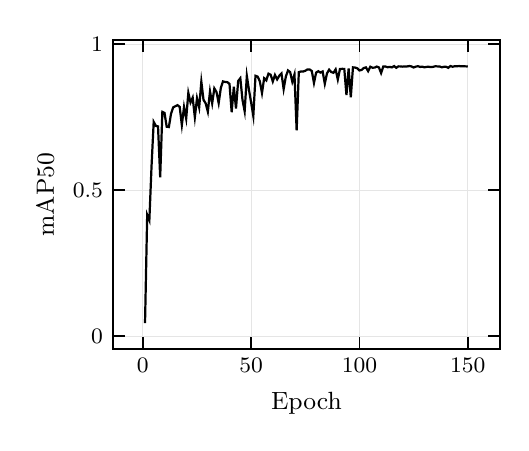
\begin{tikzpicture}
\begin{axis}[
  xlabel={Epoch},
  ylabel={mAP50},
  width=6.5cm,
  height=5.5cm,
]
\addplot[linestyle, color=black] coordinates {
  (1,0.044300)
  (2,0.415370)
  (3,0.396700)
  (4,0.580890)
  (5,0.733330)
  (6,0.719760)
  (7,0.717960)
  (8,0.543440)
  (9,0.767580)
  (10,0.763950)
  (11,0.716840)
  (12,0.715800)
  (13,0.761020)
  (14,0.782970)
  (15,0.787100)
  (16,0.790680)
  (17,0.785010)
  (18,0.722680)
  (19,0.784500)
  (20,0.744620)
  (21,0.832700)
  (22,0.799740)
  (23,0.816460)
  (24,0.749220)
  (25,0.814310)
  (26,0.782630)
  (27,0.870990)
  (28,0.808930)
  (29,0.796950)
  (30,0.768380)
  (31,0.837870)
  (32,0.796920)
  (33,0.847970)
  (34,0.835550)
  (35,0.798060)
  (36,0.849930)
  (37,0.871910)
  (38,0.870170)
  (39,0.869360)
  (40,0.863510)
  (41,0.766700)
  (42,0.853520)
  (43,0.779140)
  (44,0.873390)
  (45,0.883000)
  (46,0.808300)
  (47,0.769740)
  (48,0.890930)
  (49,0.842480)
  (50,0.799160)
  (51,0.753440)
  (52,0.891200)
  (53,0.888550)
  (54,0.872310)
  (55,0.832350)
  (56,0.882940)
  (57,0.875750)
  (58,0.898530)
  (59,0.894850)
  (60,0.871720)
  (61,0.894020)
  (62,0.878850)
  (63,0.891430)
  (64,0.899290)
  (65,0.845820)
  (66,0.888190)
  (67,0.909460)
  (68,0.903840)
  (69,0.870940)
  (70,0.895710)
  (71,0.704100)
  (72,0.903480)
  (73,0.906020)
  (74,0.905770)
  (75,0.908350)
  (76,0.913210)
  (77,0.912850)
  (78,0.907550)
  (79,0.866750)
  (80,0.902290)
  (81,0.906820)
  (82,0.902270)
  (83,0.905990)
  (84,0.864110)
  (85,0.899350)
  (86,0.912150)
  (87,0.904120)
  (88,0.901670)
  (89,0.913120)
  (90,0.878530)
  (91,0.914300)
  (92,0.915070)
  (93,0.914810)
  (94,0.824930)
  (95,0.916010)
  (96,0.817320)
  (97,0.920160)
  (98,0.919460)
  (99,0.916720)
  (100,0.909390)
  (101,0.911390)
  (102,0.917910)
  (103,0.920020)
  (104,0.907230)
  (105,0.922350)
  (106,0.919070)
  (107,0.919190)
  (108,0.922750)
  (109,0.919770)
  (110,0.900610)
  (111,0.922930)
  (112,0.923020)
  (113,0.920520)
  (114,0.921580)
  (115,0.920070)
  (116,0.924500)
  (117,0.918680)
  (118,0.923530)
  (119,0.923360)
  (120,0.922550)
  (121,0.923200)
  (122,0.923310)
  (123,0.924630)
  (124,0.923520)
  (125,0.919650)
  (126,0.922600)
  (127,0.924030)
  (128,0.921560)
  (129,0.922430)
  (130,0.920280)
  (131,0.921760)
  (132,0.922110)
  (133,0.920940)
  (134,0.921940)
  (135,0.923830)
  (136,0.923390)
  (137,0.923100)
  (138,0.920380)
  (139,0.921930)
  (140,0.922010)
  (141,0.918560)
  (142,0.924580)
  (143,0.922160)
  (144,0.924080)
  (145,0.923860)
  (146,0.924570)
  (147,0.923510)
  (148,0.924140)
  (149,0.923480)
  (150,0.923300)
};
\end{axis}
\end{tikzpicture}
\end{figure}

% YOLOv12-L DDP mAP50-95
\begin{figure}[h]
\centering
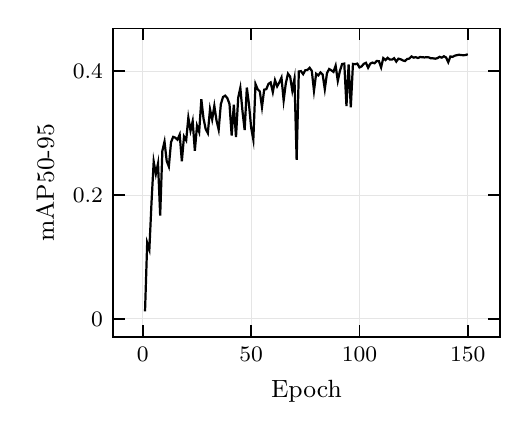
\begin{tikzpicture}
\begin{axis}[
  xlabel={Epoch},
  ylabel={mAP50-95},
  width=6.5cm,
  height=5.5cm,
]
\addplot[linestyle, color=black] coordinates {
  (1,0.012180)
  (2,0.122920)
  (3,0.111820)
  (4,0.188250)
  (5,0.253950)
  (6,0.233910)
  (7,0.250800)
  (8,0.166870)
  (9,0.271100)
  (10,0.286160)
  (11,0.255010)
  (12,0.245840)
  (13,0.285130)
  (14,0.293780)
  (15,0.292430)
  (16,0.289230)
  (17,0.297400)
  (18,0.254560)
  (19,0.294350)
  (20,0.288210)
  (21,0.324860)
  (22,0.303710)
  (23,0.319030)
  (24,0.271330)
  (25,0.311730)
  (26,0.301680)
  (27,0.354400)
  (28,0.323480)
  (29,0.306520)
  (30,0.299790)
  (31,0.338500)
  (32,0.321820)
  (33,0.343870)
  (34,0.320290)
  (35,0.305380)
  (36,0.346480)
  (37,0.358040)
  (38,0.360300)
  (39,0.356350)
  (40,0.346800)
  (41,0.296010)
  (42,0.345600)
  (43,0.293290)
  (44,0.356800)
  (45,0.372930)
  (46,0.335040)
  (47,0.304740)
  (48,0.373310)
  (49,0.346110)
  (50,0.308660)
  (51,0.289190)
  (52,0.379040)
  (53,0.370650)
  (54,0.366980)
  (55,0.341820)
  (56,0.369930)
  (57,0.370860)
  (58,0.379360)
  (59,0.381600)
  (60,0.366100)
  (61,0.385310)
  (62,0.375290)
  (63,0.381620)
  (64,0.389470)
  (65,0.352650)
  (66,0.380150)
  (67,0.395790)
  (68,0.391020)
  (69,0.368410)
  (70,0.387470)
  (71,0.256660)
  (72,0.399310)
  (73,0.399870)
  (74,0.395020)
  (75,0.401340)
  (76,0.401820)
  (77,0.405320)
  (78,0.400310)
  (79,0.368190)
  (80,0.395640)
  (81,0.392960)
  (82,0.397760)
  (83,0.394550)
  (84,0.370790)
  (85,0.396540)
  (86,0.403340)
  (87,0.401280)
  (88,0.398700)
  (89,0.408690)
  (90,0.384200)
  (91,0.400450)
  (92,0.411340)
  (93,0.412050)
  (94,0.343620)
  (95,0.410540)
  (96,0.341580)
  (97,0.411550)
  (98,0.411070)
  (99,0.412060)
  (100,0.405890)
  (101,0.407530)
  (102,0.411670)
  (103,0.413360)
  (104,0.405290)
  (105,0.411880)
  (106,0.413630)
  (107,0.412570)
  (108,0.416310)
  (109,0.415940)
  (110,0.405950)
  (111,0.420910)
  (112,0.417770)
  (113,0.421420)
  (114,0.418550)
  (115,0.418460)
  (116,0.420770)
  (117,0.415260)
  (118,0.420000)
  (119,0.419080)
  (120,0.417220)
  (121,0.416210)
  (122,0.419410)
  (123,0.420180)
  (124,0.423690)
  (125,0.421670)
  (126,0.422450)
  (127,0.421040)
  (128,0.422640)
  (129,0.422380)
  (130,0.422000)
  (131,0.422400)
  (132,0.422090)
  (133,0.420500)
  (134,0.420590)
  (135,0.419960)
  (136,0.420860)
  (137,0.423000)
  (138,0.421650)
  (139,0.423860)
  (140,0.421880)
  (141,0.414270)
  (142,0.423570)
  (143,0.422940)
  (144,0.424790)
  (145,0.425680)
  (146,0.426330)
  (147,0.425780)
  (148,0.425630)
  (149,0.425780)
  (150,0.427200)
};
\end{axis}
\end{tikzpicture}
\end{figure}



\end{document}
